\documentclass{standalone}
\usepackage[T1]{fontenc}
\usepackage[latin2]{inputenc}
\usepackage[english]{babel}
\usepackage{tikz}
\usetikzlibrary{calc,through,backgrounds,positioning,fit}
\usetikzlibrary{shapes,arrows,shadows}
 
\begin{document}
 
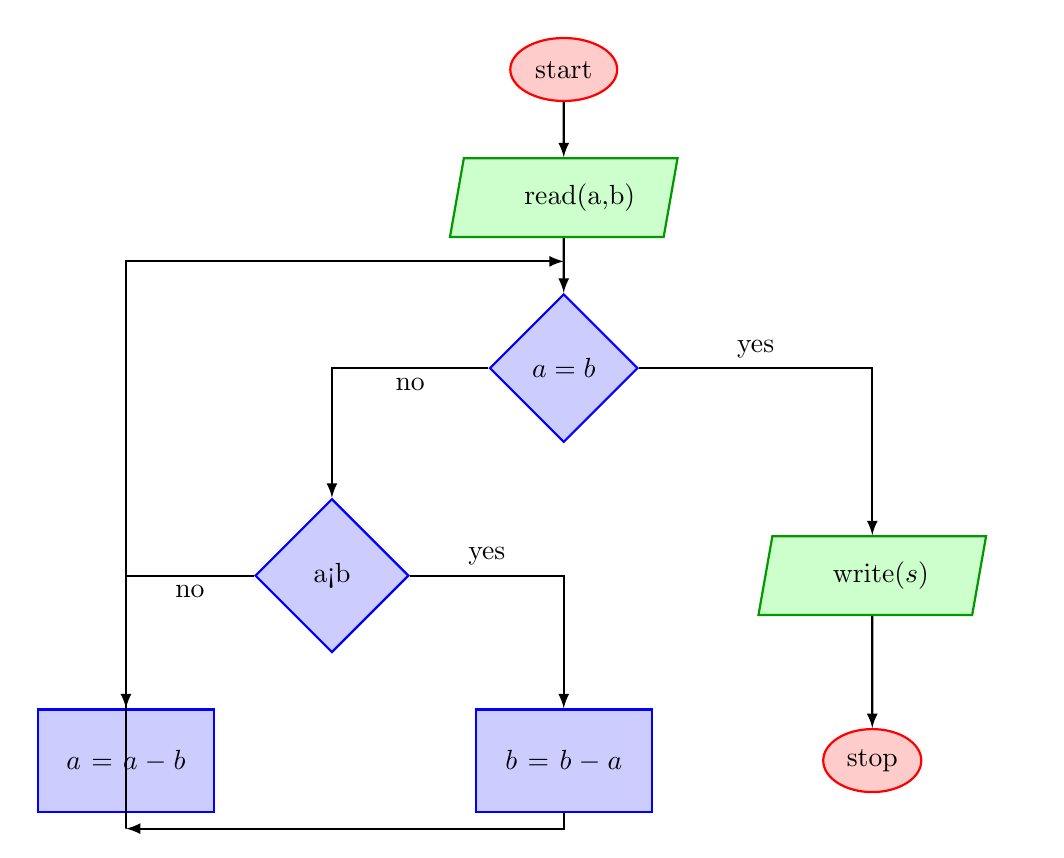
\begin{tikzpicture}[auto,
decision/.style = {diamond, draw=blue, thick, fill=blue!20, text width=1.5cm, 
                   align=flush center, inner sep=1pt},
block/.style = {rectangle, draw=blue, thick, fill=blue!20, text width=2cm, 
                align=center, minimum height=1.3cm},
start/.style = {draw=red, thick, ellipse, fill=red!20, minimum height=8mm},
inout/.style = {draw=green!60!black, thick, fill=green!20, trapezium, trapezium left angle=80, 
                trapezium right angle=-80, minimum height=10mm, text width=1cm, align=center, 
                inner sep=1pt},
line/.style ={draw, thick, -latex}]
 
\matrix[column sep=5mm,row sep=7mm]
{
% row 1
&& \node [start] (start) {start}; \\
% row 2
&& \node [inout] (read) {read(a,b)}; & \\
% row 3

% row 3
&& \node [decision] (decide) {$a = b$}; & \\
% row 4
&\node [decision] (decider) {a<b}; &&
& \node [inout] (write) {write($s$)}; & \\
% row 5
\node [block] (init) {$a=a-b$}; 
&& \node [block] (initt) {$b=b-a$}; 
&& \node [start] (stop) {stop}; \\
};
 
\begin{scope}[every path/.style=line]
\path (start) -- (read);
\path (read) -- (decide);
\path (decide) -| node [near start] {yes} (write);
\path (decide) -| node [near start] {no} (decider);
\path (decider) -| node [near start] {yes} (initt);
\path (decider) -| node [near start] {no} (init);
\path (write) -- (stop);
\path (init.south) -- ++(0,-0.2)  |- ($ (decide.north) + (0,0.4) $);
\path (initt.south) -- ++(0,-0.2) |- ($ (init.south) + (0,-0.2) $);
\end{scope}
\end{tikzpicture}
\end{document}